% ============================================================
%  QSP Clock Protocol  —  PRA-style manuscript
%  Restructured: clock-performance-centric narrative
% ============================================================
\documentclass[aps,pra,twocolumn,superscriptaddress,longbibliography]{revtex4-2}

\usepackage{amsmath,amssymb,mathtools}
\usepackage{graphicx}
\usepackage{bm}
\usepackage{physics}
\usepackage{xcolor}
\usepackage{hyperref}
\usepackage{cleveref}
\usepackage{float}
\usepackage[normalem]{ulem}
\usepackage{caption}
\usepackage{booktabs}

% ------ custom macros ------
\newcommand{\bb}[1]{\mathbf{#1}}
\newcommand{\id}{\mathbb{I}}
\newcommand{\w}{\omega}
\newcommand{\rabi}{\Omega}
\newcommand{\be}{\begin{equation}}
\newcommand{\ee}{\end{equation}}
\newtheorem{theorem}{Theorem}

% placeholder color
\newcommand{\placeholder}[1]{{\color{red}\textbf{[PLACEHOLDER: #1]}}}
\newcommand{\todo}[1]{{\color{blue}\textbf{[TODO: #1]}}}

\graphicspath{{figures/qubit_performance_plots/}}

\begin{document}

\title{Noise-Resilient Atomic Clocks via Quantum Signal Processing:\\
       Sensitivity, Filtering, and Multilevel Spectroscopy}

\author{Author One}
\affiliation{Department of Physics, Institution A}
\author{Author Two}
\affiliation{Department of Physics, Institution B}

\date{\today}

\begin{abstract}
We develop a unified analytical framework for characterizing and optimizing atomic clock performance
under realistic noise environments using Quantum Signal Processing (QSP).
Clock performance is governed by two competing figures of merit:
the \emph{frequency sensitivity} $\mathcal{S}^2 = |\partial_\delta\langle M\rangle|^2$,
which quantifies how steeply the atomic signal discriminates a frequency deviation $\delta$
from resonance, and the \emph{Kubo noise integral}
$\mathcal{K}(S_\beta) = \int S_\beta(\omega)\mathcal{F}_e(\omega)\,d\omega/(2\pi)$,
which measures how strongly the pulse sequence couples to off-resonant technical noise.
Maximizing clock stability requires simultaneously maximizing $\mathcal{S}^2$ and minimizing
$\mathcal{K}$, making the figure of merit $\mathrm{FOM}=\mathcal{S}^2/\mathcal{K}$ the central
optimization target.
We show that the physically correct laser-detuning Hamiltonian $H_\delta = \delta|e\rangle\langle e|$
leads to an analytic result: \emph{all} GPS protocols at integer-cycle resonance ($\delta=0$) share
the same DC sensitivity $|\partial_\delta S|^2 = T^2/4$ as Ramsey, so protocol differences reduce
entirely to filter-function differences.
Within the equiangular protocol class (continuous $N$-segment drives), numerical optimization of the
FOM shows at most $15\%$ improvement over Ramsey for white noise; GPS $m=1$ is nearly optimal
for band-limited (high-pass) noise environments where its filter function is concentrated below
the noise cutoff.
Crucially, pulsed QSP sequences consisting of $n$ fast rotations separated by equal free-evolution
gaps---analogous to CPMG dynamical-decoupling sequences---achieve $3$--$7\times$ improvement in FOM
over all continuous-drive protocols for white and $1/f$ noise, by suppressing low-frequency noise
via partial spin-echo refocusing while maintaining finite sensitivity.
These results are validated via exact numerical filter-function calculations and establish a
quantitative hierarchy of clock protocols matched to the noise environment.
\end{abstract}

\maketitle

% ============================================================
\section{Introduction}
\label{sec:intro}
% ============================================================

Optical atomic clocks have reached unprecedented levels of precision, with systematic
uncertainties at or below the $10^{-18}$ level \cite{}.
Yet further improvements---particularly for portable and fieldable clocks---require confronting
two practical challenges that are not fully addressed by the standard two-level Ramsey protocol:
(i) maximizing the \emph{DC sensitivity} of the atomic response so that small frequency
deviations produce large, resolvable signal changes, and
(ii) suppressing \emph{fast frequency noise} (laser phase noise, magnetic field fluctuations,
vibrations) that falls within the bandwidth of the interrogation sequence.
Both challenges are ultimately questions about how a quantum system processes and filters
its environment, and both can be addressed through careful design of the pulse sequence
applied to the atomic transition.

Quantum Signal Processing (QSP) \cite{} provides a systematic algebraic framework for
designing pulse sequences that implement prescribed polynomial transformations of quantum
matrix elements \cite{}.
Although QSP was originally introduced in the context of quantum algorithms,
its structure---alternating between a fixed ``signal'' rotation and programmable
``signal processing'' phase shifts---maps naturally onto the composite pulse sequences
already used in atomic physics (Ramsey, CPMG, hyper-Ramsey, dynamical decoupling).
This suggests that QSP provides a unifying language for understanding and optimizing
the noise-filtering properties of clock protocols.

Prior work has analyzed composite pulse sequences for clocks using the
filter-function formalism \cite{Cywinski2008,Green2013,Soare2014},
and dynamical decoupling sequences have been demonstrated to suppress dephasing noise
in atomic systems \cite{Biercuk2009,Bylander2011}.
However, these approaches typically treat pulses as instantaneous, neglecting
the finite duration of the drive and the correlated noise experienced \emph{during}
each pulse.
Furthermore, they do not directly connect to the per-shot frequency sensitivity
$\sigma^2_\nu$ that governs clock stability.
The GPS protocol \cite{GPS} introduced measurement via a three-level $\Lambda$ system to improve
sensitivity, but a theoretical framework connecting GPS to filter function design is lacking.

In this work, we close these gaps by developing the \emph{temporal QSP} formalism:
an extension of canonical QSP to continuous-time noise processes that captures
both finite-pulse-duration effects and the full spectral structure of the noise.
Our main contributions are:

\begin{enumerate}
  \item A unified analytical expression for the per-shot frequency sensitivity and
        noise filter function in terms of temporal QSP polynomials $F(t),G(t)$,
        valid for both two-level and three-level $\Lambda$-system clocks
        (Secs.~\ref{sec:temporal_qsp}--\ref{sec:multilevel}).

  \item An analytic proof that \emph{all} GPS protocols operating at integer-cycle resonance
        ($\delta=0$) share the same DC sensitivity as Ramsey: $|\partial_\delta S|^2 = T^2/4$,
        so protocol differences in FOM arise entirely from filter-function differences
        (Sec.~\ref{sec:gps}).

  \item A demonstration that GPS filter functions are \emph{peaked}, not nulled, at the Rabi
        frequency; GPS $m=1$ achieves near-perfect noise rejection for band-limited noise
        with cutoff above $\Omega = 2\pi m/T$ (Sec.~\ref{sec:analytics}).

  \item A systematic comparison of three protocol classes under white, $1/f$, and high-pass
        noise: continuous-drive GPS, optimized equiangular, and pulsed QSP sequences
        (Sec.~\ref{sec:analytics}).

  \item The discovery that pulsed QSP sequences---optimized over rotation angles and phases
        under a fixed fast Rabi frequency---rediscover CPMG-like spin-echo structures that
        achieve $3$--$7\times$ FOM improvement over all continuous-drive protocols by
        suppressing low-frequency noise via partial spin-echo refocusing
        (Sec.~\ref{sec:analytics}).

  \item Analytical conditions under which the Kubo linear response approximation holds,
        with numerical verification (Sec.~\ref{sec:validity}).
\end{enumerate}

The paper is organized as follows.
Section~\ref{sec:metrics} introduces the two key clock performance metrics and the FOM.
Section~\ref{sec:temporal_qsp} develops the temporal QSP formalism and Kubo linear
response theory for the three-level $\Lambda$ clock.
Section~\ref{sec:multilevel} analyzes two-level and three-level protocols, establishing
the GPS sensitivity formula and filter function structure.
Section~\ref{sec:analytics} presents the full protocol comparison and figures.
Section~\ref{sec:validity} analyzes the validity regime of linear response theory.
Section~\ref{sec:pulseshaping} discusses pulse shaping to further optimize noise filtering.
Section~\ref{sec:strong_noise} addresses the strongly noisy regime via direct clock
simulations and Allan variance.
We conclude in Section~\ref{sec:conclusion}.


% ============================================================
\section{Clock Performance Metrics}
\label{sec:metrics}
% ============================================================

This section defines the two key figures of merit that quantify atomic clock performance
and establishes the FOM that combines them into a single optimization target.
We will show that these two quantities---sensitivity and noise---are both controlled by
the same underlying object, the temporal QSP path function $\Phi(t)$, which connects
the clock design problem to the algebra of SU(2) rotations.

\subsection{Frequency sensitivity}
\label{sec:freq_sensitivity}

A clock operates by measuring an observable $M$ that depends on the laser-atom detuning
$\delta$, and feeding the result back to correct the local oscillator.
The quality of a single measurement is captured by the \emph{per-shot frequency sensitivity}:
\be
  \sigma^2_\nu(\delta) \equiv \frac{\mathrm{Var}(M)}{|\partial_\delta \langle M \rangle|^2}\,,
  \label{eq:sigma_nu}
\ee
which is the variance of the measured signal divided by the square of the slope of the
mean signal with respect to detuning.
This has units of frequency$^2$: it is the minimum frequency deviation detectable
in a single shot, and it is what the clock servo directly minimizes.

On resonance ($\delta = 0$), the numerator has two contributions:
\be
  \mathrm{Var}(M) = \mathrm{Var}_{\rm QPN}(M) + \langle \delta M^2 \rangle_{\rm noise}\,,
  \label{eq:var_total}
\ee
where $\mathrm{Var}_{\rm QPN}$ is quantum projection noise (irreducible) and
$\langle \delta M^2 \rangle_{\rm noise}$ is the variance driven by technical noise.
Good clock design means both \emph{maximizing the signal slope}
$\mathcal{S} = |\partial_\delta\langle M\rangle|_{\delta=0}$ and
\emph{minimizing the noise variance} $\langle\delta M^2\rangle_{\rm noise}$.

For wide-sense stationary technical noise, the Kubo linear response formula gives
\be
  \langle \delta M^2 \rangle_{\rm noise} = \int_{-\infty}^{\infty}
    \frac{d\omega}{2\pi}\, S_\beta(\omega)\, \mathcal{F}_e(\omega)\,,
  \label{eq:noise_var_general}
\ee
where $S_\beta(\omega)$ is the (one-sided) noise power spectral density and $\mathcal{F}_e(\omega)$
is the \emph{filter function} of the pulse sequence, derived in Sec.~\ref{sec:temporal_qsp}.
The filter function is entirely determined by the trajectory of the quantum state during
the pulse sequence: different protocols (Ramsey, GPS, CPMG, equiangular) differ only in
the shape of this trajectory.

\subsection{Figure of merit}
\label{sec:fom}

The two metrics---sensitivity $\mathcal{S}^2$ and noise Kubo integral
$\mathcal{K}(S_\beta) = \int \mathcal{F}_e(\omega)S_\beta(\omega)\,d\omega/(2\pi)$---combine
into a single \emph{figure of merit} (FOM):
\be
  \mathrm{FOM}(S_\beta) \equiv \frac{\mathcal{S}^2}{\mathcal{K}(S_\beta)}
  = \frac{|\partial_\delta\langle M\rangle|^2_{\delta=0}}
         {\displaystyle\int_{-\infty}^\infty \frac{d\omega}{2\pi}\,S_\beta(\omega)\,\mathcal{F}_e(\omega)}\,.
  \label{eq:fom}
\ee
Maximizing FOM is equivalent to minimizing the per-shot frequency estimation variance
$\sigma^2_\nu$.  The FOM depends on the noise model: different noise spectra $S_\beta(\omega)$
favor different protocol designs.

Throughout this paper we compare protocols under three noise models of practical importance:
\begin{enumerate}
  \item \emph{White noise}: $S(\omega) = S_0$, modeling short-timescale LO instability.
  \item \emph{$1/f$ noise}: $S(\omega) = S_0/|\omega|$, modeling low-frequency flicker noise.
  \item \emph{High-pass noise}: $S(\omega) = S_0\,\Theta(|\omega| - \omega_c)$ with
        $\omega_c = 2$\,rad/s, modeling a noise floor that exists only above a $1/f$ corner
        frequency.
\end{enumerate}
For $1/f^\alpha$ noise environments, the noise power is concentrated at low frequencies and
falls with increasing $\omega$.  The overlap integral~\eqref{eq:noise_var_general} is then
minimized by making $\mathcal{F}_e(\omega)$ small at low frequencies.
For high-pass environments, a protocol whose filter function is concentrated \emph{below}
the cutoff $\omega_c$ achieves nearly perfect noise rejection.
The relationship between FOM and the Allan deviation $\sigma_y(\tau)$ is established
in Sec.~\ref{sec:strong_noise}.


% ============================================================
\section{Temporal QSP and Kubo Linear Response}
\label{sec:temporal_qsp}
% ============================================================

This section develops the mathematical framework used throughout the paper.
We define the temporal QSP polynomial trajectory, derive the Kubo formula for the noise
variance in terms of this trajectory, and specialize to the three-level $\Lambda$ clock.
The key output is the filter function $\mathcal{F}_e(\omega)$ of~\eqref{eq:noise_var_general},
which is evaluated for each protocol in Sec.~\ref{sec:analytics}.

\subsection{The temporal QSP formalism}
\label{sec:tqsp_formalism}

A general pulse sequence consists of $d$ segments, each a continuous drive at Rabi frequency
$\Omega_j$ and phase $\phi_j$ for duration $\tau_j$ (total time $T = \sum_j\tau_j$).
Written in the $2\times 2$ SU(2) representation of the probe subspace
$\{|g\rangle,|e\rangle\}$, the propagator at time $t$ during segment $j$ is:
\begin{align}
  U_{\rm QSP}(t) &\equiv \begin{pmatrix} F(t) & iG(t) \\ iG^*(t) & F^*(t) \end{pmatrix}
  \label{eq:u_qsp_poly}
\end{align}
where the Cayley--Klein amplitudes $F(t), G(t)$ satisfy $|F|^2+|G|^2=1$ and obey the
recurrence (see Appendix~\ref{app:recurrences})
\begin{align}
  F_j(t) &= \cos\tfrac{\theta_j(t)}{2}\,f_{j-1} - e^{-i\phi_j}\sin\tfrac{\theta_j(t)}{2}\,g_{j-1}^*\,,
  \label{eq:recurrence_F} \\
  G_j(t) &= \cos\tfrac{\theta_j(t)}{2}\,g_{j-1} + e^{-i\phi_j}\sin\tfrac{\theta_j(t)}{2}\,f_{j-1}^*\,,
  \label{eq:recurrence_G}
\end{align}
with $\theta_j(t) = \Omega_j(t - t_{j-1})$, $f_0 = 1$, $g_0 = 0$.

The global Cayley--Klein amplitudes $F(t)$, $G(t)$ are assembled piecewise from these
per-segment solutions.  Defining segment boundaries $t_j = \sum_{k=1}^j\tau_k$
(with $t_0=0$, $t_d=T$), the Heaviside step function $\Theta$ selects the active segment
at each time $t$:
\begin{align}
  F(t) &= \sum_{j=1}^{d} F_j(t-t_{j-1})\,\bigl[\Theta(t-t_{j-1})-\Theta(t-t_j)\bigr]\,,
  \label{eq:F_piecewise}\\
  G(t) &= \sum_{j=1}^{d} G_j(t-t_{j-1})\,\bigl[\Theta(t-t_{j-1})-\Theta(t-t_j)\bigr]\,,
  \label{eq:G_piecewise}
\end{align}
where each $F_j(\cdot)$, $G_j(\cdot)$ satisfies~\eqref{eq:recurrence_F}--\eqref{eq:recurrence_G}
with initial conditions $(f_{j-1},\,g_{j-1})$ at the start of segment $j$.
The Fourier integrals~\eqref{eq:Phi}--\eqref{eq:Chi} then decompose into a sum of
$d$ segment contributions, each evaluated over $[t_{j-1},t_j]$.

The within-segment behavior of $F_j(t)$, $G_j(t)$ depends on the protocol class
and gives rise to two qualitatively different recurrences:
\begin{description}
  \item[Equiangular] Continuous drives ($\Omega_j\neq 0$) give
        $\theta_j(t)=\Omega_j(t-t_{j-1})$ growing linearly in $t$, so $F_j$, $G_j$
        trace smooth arcs on the SU(2) manifold throughout each segment.
  \item[Pulsed QSP] Free-evolution segments have $\Omega_j=0$, so $\theta_j(t)=0$
        throughout.  Equations~\eqref{eq:recurrence_F}--\eqref{eq:recurrence_G}
        then reduce to $F_j(t)=f_{j-1}$ and $G_j(t)=g_{j-1}$ (constant):
        the amplitudes remain frozen between instantaneous rotation pulses.
\end{description}

Two scalar path functions encode the noise-filtering properties:
\be
  \phi(t) = F^*(t)G(t)\,,\qquad \chi(t) = |G(t)|^2\,,
  \label{eq:path_functions}
\ee
and their Fourier transforms:
\begin{align}
  \Phi(\omega) &= \int_0^T F^*(t)G(t)\,e^{-i\omega t}\,dt\,,
  \label{eq:Phi} \\
  \mathcal{X}(\omega) &= \int_0^T |G(t)|^2\,e^{-i\omega t}\,dt\,.
  \label{eq:Chi}
\end{align}
The shape of the path $t\mapsto (F(t),G(t))$ on the SU(2) manifold---not just its endpoint---determines
the filter function.

\subsubsection{Pulsed QSP protocol}
\label{sec:qsp_pulsed}

A pulsed QSP sequence consists of $n$ instantaneous rotations
$R(\theta_j, \phi_j)$ in the $xy$-plane, separated by $n-1$ equal free-evolution gaps:
\be
  R(\theta_1,\phi_1) - \tau_{\rm free} - R(\theta_2,\phi_2) - \cdots - R(\theta_n,\phi_n)\,,
  \label{eq:qsp_pulsed}
\ee
with $\tau_{\rm free} = (T - \sum_j\tau_j)/(n-1)$ and fast pulses $\tau_j = \theta_j/\Omega_{\rm fast}$
($\Omega_{\rm fast} = 20\pi$) short compared to $\tau_{\rm free}$.
The $2n-1$ free parameters are $\theta_1,\ldots,\theta_n\in(0,\pi]$ and
$\phi_2,\ldots,\phi_n\in[0,2\pi)$ ($\phi_1=0$ by gauge).
Ramsey is the special case $n=2$, $\theta_j = \pi/2$, $\phi_j = 0$.

Because the free-evolution segments satisfy $F_j(t)=f_{j-1}$ and $G_j(t)=g_{j-1}$ (constant),
the path functions $\phi(t)=F^*G$ and $\chi(t)=|G|^2$ are piecewise constant between pulses.
Each instantaneous rotation steps them to a new constant value via the SU(2)
recurrence~\eqref{eq:recurrence_F}--\eqref{eq:recurrence_G} at zero duration.
The Fourier integrals~\eqref{eq:Phi}--\eqref{eq:Chi} therefore reduce to a sum of
sinc-like terms, one per free-evolution gap.

These sequences are optimized using the same procedure as equiangular (see Appendix~\ref{app:optimization}).
For $n=3,5,9$, the optimizer consistently finds sequences with a final pulse of
$\theta_n \approx 0.85$--$0.92\pi$, a near-$\pi$ refocusing pulse that creates a
partial spin echo.  Performance is compared in Sec.~\ref{sec:analytics}.

\paragraph{Noise Hamiltonian for the $\Lambda$ system.}
The dominant noise source is a stochastic detuning fluctuation:
\be
  H_\epsilon(t) = \beta_e(t)\,|e\rangle\langle e|\,,
  \label{eq:noise_ham_3L}
\ee
where $\beta_e(t)$ represents laser frequency noise modeled as a zero-mean,
wide-sense stationary Gaussian process with PSD $S_{\beta_e}(\omega)$.
Magnetic field noise on the clock transition $|g\rangle$-$|m\rangle$ is included
via the $\mathcal{F}_m$ term in~\eqref{eq:main_result} but neglected below.


\subsection{Three-level $\Lambda$-clock propagator}
\label{sec:3level_propagator}

For the three-level $\Lambda$ system with states $|g\rangle$, $|e\rangle$, $|m\rangle$,
the physically correct laser-detuning Hamiltonian is
\be
  H_\delta = \delta\,|e\rangle\langle e|\,,
  \label{eq:H_delta}
\ee
which shifts only the optically excited state (not $|g\rangle$ or $|m\rangle$).
This is \emph{not} traceless in the probe subspace; ignoring the difference leads to
incorrect signal predictions for multi-segment sequences (see Appendix~\ref{app:gps_sensitivity}).

Under a continuous drive at Rabi frequency $\Omega$ and detuning $\delta$ for duration $\tau$,
the three-level propagator is
\be
  U(\tau) = e^{-i\delta\tau/2}
  \begin{pmatrix}
      f & ig & 0 \\
      ig^* & f^* & 0 \\
      0 & 0 & e^{+i\delta\tau/2}
  \end{pmatrix},
  \label{eq:propagator_3L}
\ee
where $f,g$ are the CK amplitudes for the SU(2) rotation in the probe subspace under
the \emph{traceless} part of $H_\delta + H_{\rm drive}$, and the global probe phase
$e^{-i\delta\tau/2}$ accumulates relative to $|m\rangle$ across each segment.
For multi-segment sequences, this global phase must be tracked cumulatively.

\subsection{Kubo linear response and the filter function}
\label{sec:kubo}

We compute the noise-driven variance in the toggling frame of the QSP sequence.
With initial state $|\Psi\rangle = (|g\rangle + |m\rangle)/\sqrt{2}$ and observable
$M = \sigma_y^{gm} = -i|g\rangle\langle m| + i|m\rangle\langle g|$
(corresponding to measurement direction $\hat{y}$ in the $\{g,m\}$ Bloch sphere,
with $m_y=1$, $m_x=m_z=0$), the Kubo formula evaluates to (derived in Appendix~\ref{app:kubo}):
\be
  \langle \delta M^2 \rangle = \int_{-\infty}^{\infty}\frac{d\omega}{2\pi}
    \Bigl[S_{\beta_e}(\omega)\,\mathcal{F}_e(\omega) + S_{\beta_m}(\omega)\,\mathcal{F}_m(\omega)\Bigr]\,,
  \label{eq:main_result}
\ee
with the e-noise and m-noise filter functions:
\begin{align}
  \mathcal{F}_e(\omega) &= \tfrac{1}{2}|\Phi(\omega)|^2 + |\mathcal{X}(\omega)|^2\,,
  \label{eq:Fe} \\
  \mathcal{F}_m(\omega) &= -\frac{1 - \cos\omega T}{\omega^2}\,,
  \label{eq:Fm}
\end{align}
where $\Phi(\omega)$ and $\mathcal{X}(\omega)$ are defined in~\eqref{eq:Phi}--\eqref{eq:Chi}.

The filter function $\mathcal{F}_e(\omega)$ is composed of two terms:
$\frac{1}{2}|\Phi|^2$ from the coherence channel $F^*G$ (coupling of e-noise to the
$|g\rangle$-$|e\rangle$ coherence) and $|\mathcal{X}|^2$ from the population channel $|G|^2$
(coupling to the $|e\rangle$ population).
For a pure free-evolution segment at $\delta=0$, $F$ and $G$ are constant, and neither
channel accumulates noise; noise enters only during the driven segments.
The $\mathcal{F}_m$ term describes noise on the clock transition $|g\rangle$-$|m\rangle$;
for optical clocks with a stable RF reference, $S_{\beta_m} \ll S_{\beta_e}$ and this
term is negligible.  We therefore focus on $\mathcal{F}_e$ throughout.

\subsection{Signal slope}
\label{sec:kubo_dc}

The signal slope $\mathcal{S} = \partial_\delta\langle M\rangle|_{\delta=0}$ is computed
from the detuning derivative of the propagator~\eqref{eq:propagator_3L}.
Both the global probe phase and the detuning dependence of the CK amplitudes contribute.
The analytic formula for GPS protocols is derived in Appendix~\ref{app:gps_sensitivity};
for general sequences, $\mathcal{S}$ is evaluated numerically.


% ============================================================
\section{Two-Level vs.\ Three-Level Systems}
\label{sec:multilevel}
% ============================================================

This section uses the temporal QSP framework to compare two-level Ramsey spectroscopy
with three-level GPS and equiangular protocols.
A central result---Eq.~\eqref{eq:gps_sens_result}---is that all GPS protocols at
integer-cycle resonance share the same DC sensitivity as Ramsey, reducing the
protocol comparison entirely to filter-function differences.
We also clarify the structure of GPS filter functions, correcting a common misstatement
that GPS has filter-function nulls at the Rabi harmonics.

\subsection{Two-level spectroscopy}
\label{sec:two-level}

For a two-level atom ($|m\rangle$ identified with $|e\rangle$, $M = \sigma_z$),
the filter function reduces to $\mathcal{F}^{(2L)}(\omega) = |\Phi(\omega)|^2$
(see Appendix~\ref{app:two_level_reduction}).

\subsubsection{Ramsey}
\label{sec:ramsey}

The standard Ramsey protocol consists of two $\pi/2$ pulses of duration $\tau_p = \pi/(2\Omega_{\rm fast})$
separated by free precession of duration $\tau_{\rm free} = T - 2\tau_p$.
For $\Omega_{\rm fast} T \gg 1$ (fast-pulse limit), the filter function for instantaneous pulses is
\be
  \mathcal{F}^{(2L)}_{\rm Ramsey}(\omega) = \frac{4\sin^2(\omega T/2)}{\omega^2}\,,
  \label{eq:F_ramsey}
\ee
with high-frequency roll-off $\mathcal{F} \sim \omega^{-2}$.
The slope is $\mathcal{S}_{\rm Ramsey} = T/2$, giving
$|\mathcal{S}_{\rm Ramsey}|^2 = T^2/4 = \pi^2$ for $T=2\pi$.

\subsection{Three-level spectroscopy}
\label{sec:gps}

Global Phase Spectroscopy (GPS) \cite{GPS} uses a three-level $\Lambda$ system
with states $|g\rangle$, $|e\rangle$, $|m\rangle$, where:
\begin{itemize}
  \item $|g\rangle \leftrightarrow |e\rangle$: optical probe transition driven by the clock laser.
  \item $|g\rangle \leftrightarrow |m\rangle$: RF (M1) clock transition with long coherence time,
        used for readout via $M = \sigma_y^{gm}$.
\end{itemize}
The initial state is $|\Psi_0\rangle = (|g\rangle + |m\rangle)/\sqrt{2}$.

\subsubsection{GPS protocol and signal}

The GPS-$m$ sequence consists of a single continuous resonant drive at Rabi frequency
$\Omega = 2\pi m/T$ for time $T$ (so that $\Omega T = 2\pi m$, an integer number of
complete Rabi cycles).
With the correct Hamiltonian $H_\delta = \delta|e\rangle\langle e|$, the three-level clock
signal is \cite{} (see Appendix~\ref{app:gps_sensitivity}):
\begin{align}
  S(\delta) &= \sin\!\left(\frac{\delta T}{2}\right)\cos\!\left(\frac{\Omega_R T}{2}\right)
            \nonumber \\
            &\quad - \frac{\delta}{\Omega_R}\cos\!\left(\frac{\delta T}{2}\right)
              \sin\!\left(\frac{\Omega_R T}{2}\right)\,,
  \label{eq:gps_signal}
\end{align}
where $\Omega_R = \sqrt{\Omega^2 + \delta^2}$.
This differs from the probe-subspace-traceless formula; the two agree only at $\delta = 0$
where both vanish.  All protocols here operate at $\delta = 0$ (the quadrature point).

\subsubsection{All GPS protocols share the same DC sensitivity at $\delta=0$}
\label{sec:gps_sens}

Differentiating~\eqref{eq:gps_signal} and evaluating at $\delta=0$ (where $\Omega_R = \Omega$):
\be
  \partial_\delta S\big|_{\delta=0}
  = \frac{T\,\Omega\,\cos(\Omega T/2) - 2\sin(\Omega T/2)}{2\Omega}\,.
  \label{eq:gps_deriv}
\ee
For GPS-$m$ with $\Omega T = 2\pi m$, we have $\sin(m\pi) = 0$ and $\cos(m\pi) = (-1)^m$, so
\be
  \partial_\delta S\big|_{\delta=0}
  = \frac{(-1)^m\, T}{2}\,,
  \qquad
  |\partial_\delta S|^2 = \frac{T^2}{4} = \pi^2
  \quad\forall\, m\,.
  \label{eq:gps_sens_result}
\ee
\emph{All GPS protocols at $\delta=0$ have the same DC sensitivity as Ramsey.}
The numerical values confirm this: for $T=2\pi$, all protocols give
$|\mathcal{S}|^2 \approx \pi^2 \approx 9.87$ (Table~\ref{tab:fom}).
Protocol differences in FOM therefore arise \emph{entirely} from differences in
$\mathcal{K}(S_\beta)$, not from $\mathcal{S}^2$.

\subsubsection{GPS filter function structure}
\label{sec:gps_ff}

At $\delta=0$, the CK amplitudes for a GPS-$m$ drive evolve as
$f(t) = \cos(\Omega t/2)$, $g(t) = -i\sin(\Omega t/2)$.
The two path functions are $\phi(t) = F^*G = -i\cos(\Omega t/2)\sin(\Omega t/2)$
and $\chi(t) = |G|^2 = \sin^2(\Omega t/2)$.
The Fourier transforms give:
\begin{align}
  |\Phi(\omega)|^2 &\sim T^2/4\quad(\omega\to 0)\,,\text{ decreasing to zero above }\omega\sim\Omega\,,\\
  |\mathcal{X}(\omega)|^2 &\sim \text{peaked at }\omega = \Omega\,,
\end{align}
so the GPS filter function $\mathcal{F}_e = \frac{1}{2}|\Phi|^2 + |\mathcal{X}|^2$ has a
\emph{peak} at the Rabi frequency $\omega = \Omega$, not a null.
This is a key clarification: previous analyses using the probe-subspace-traceless Hamiltonian
predicted nulls at Rabi harmonics; these nulls disappear under the correct Hamiltonian.
As a consequence, GPS-$m$ is \emph{most sensitive} to noise near $\omega\approx\Omega$, not
suppressed there.

For GPS-$m$ compared to Ramsey under white noise:
\begin{itemize}
  \item GPS-$m$ concentrates $\mathcal{F}_e$ near $\omega=\Omega$ (the Rabi frequency),
        while Ramsey has a broad $\omega^{-2}$ fall-off from low frequency.
  \item For $m=1$ ($\Omega=1$) and $m=8$ ($\Omega=8$), the Kubo integrals under white
        noise are $\mathcal{K}_w \approx 0.99$ and $1.01$, compared to Ramsey's $0.63$.
        This gives GPS FOMs of $\approx 10$ vs.\ Ramsey's $15.6$.
  \item Under $1/f$ noise, GPS-$8$ is more competitive ($\mathrm{FOM}_{1/f}=9.9$) than
        GPS-$1$ ($5.4$) because the $1/f$ noise weight at $\omega=8$ is eight times smaller
        than at $\omega=1$.
\end{itemize}

\subsection{Equiangular $N$-segment sequences}
\label{sec:equiangular}

The equiangular protocol generalizes GPS by dividing $T$ into $N$ equal segments of duration
$\tau = T/N$, each a continuous drive at shared Rabi frequency $\Omega$ with independently
optimized drive phases $\phi_k$:
\be
  \prod_{k=1}^{N} e^{-i(\Omega\tau/2)(\cos\phi_k\,\sigma_x + \sin\phi_k\,\sigma_y)}\,.
  \label{eq:eq_seq}
\ee
GPS-$m$ is the special case $N=1$ (or $N=4$ with all $\phi_k$ equal).
The free parameters $(\Omega, \phi_2,\ldots,\phi_N)$ are optimized to maximize
$\mathrm{FOM}$ for a given noise model using differential evolution followed by L-BFGS-B
polishing (described in Appendix~\ref{app:optimization}).

For $N=4$ optimized under white noise, the numerical optimum is
$\Omega T \approx 7.6$ with phases $\phi^* \approx [0, 1.44, 0.38, 1.11]$\,rad,
giving $\mathrm{FOM}_w = 14.1$---about $10\%$ below Ramsey's $15.6$.
The Rabi frequency $\Omega T \approx 7.6$ places the $\mathcal{F}_e$ peak
slightly below $\omega=2$, reducing the low-frequency noise integral while maintaining sensitivity.

% ============================================================
\section{Protocol Comparison}
\label{sec:analytics}
% ============================================================

This section presents the full numerical comparison of clock protocols under three
noise models.  All filter functions are computed via FFT of the temporal QSP path
functions $\phi(t) = F^*(t)G(t)$ and $\chi(t) = |G(t)|^2$ over the time grid
$t_k = k\,T/N_{\rm FFT}$ ($N_{\rm FFT}=4096$, zero-padded by $\times 4$).

\subsection{Filter functions}

Figure~\ref{fig:filter_functions} shows $\mathcal{F}_e(\omega)/T^2$ for all protocols
at $\delta=0$, $T=2\pi$.
The qualitative structure matches the analytic predictions of Sec.~\ref{sec:gps_ff}:
\begin{itemize}
  \item \textbf{Ramsey} has a broad, nearly flat $\mathcal{F}_e\approx T^2/4$ at low frequencies,
        with $\omega^{-2}$ roll-off above $\omega\sim 1/\tau_{\rm free}$.
  \item \textbf{GPS $m=1$} ($\Omega=1$) has $\mathcal{F}_e$ concentrated near $\omega=1$
        with very little weight above $\omega\approx 4$.
  \item \textbf{GPS $m=8$} ($\Omega=8$) has $\mathcal{F}_e$ peaked at $\omega=8$
        and its first harmonic $\omega=16$; significant weight also exists at intermediate
        frequencies $1\lesssim\omega\lesssim 8$.
  \item \textbf{Equiangular $N=4$} (white-noise optimized) sits below Ramsey across
        the mid-frequency range $0.3\lesssim\omega\lesssim 5$, giving a smaller
        $\mathcal{K}_w$ than all GPS protocols but not as good as Ramsey itself.
\end{itemize}

\begin{figure}[t]
  \centering
  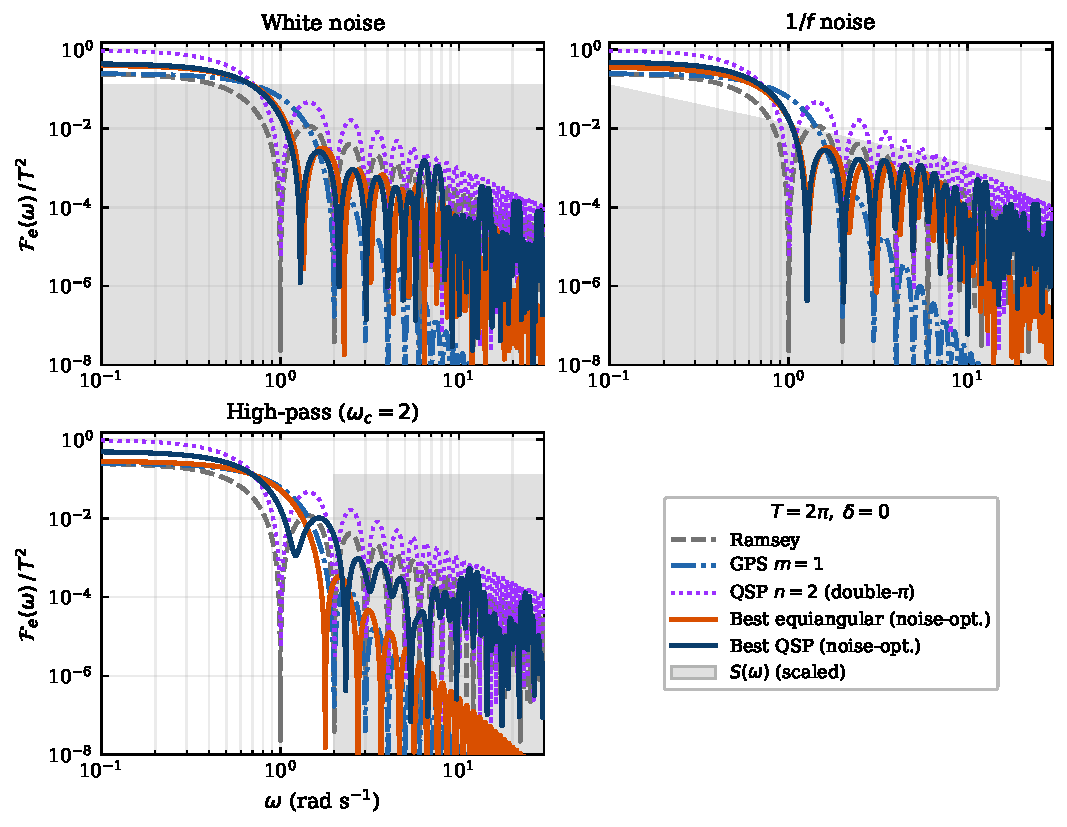
\includegraphics[width=\columnwidth]{protocol_comparison.pdf}
  \caption{%
    Filter functions $\mathcal{F}_e(\omega)/T^2$ for the four reference protocols
    at $T=2\pi$, $\delta=0$.
    Vertical dotted lines mark the Rabi harmonics of GPS $m=1$ (blue) and GPS $m=8$ (green).
    GPS $\mathcal{F}_e$ is \emph{peaked} at the Rabi frequency, not nulled.
    Computed via Eqs.~\eqref{eq:Fe}--\eqref{eq:Chi}.%
  }
  \label{fig:filter_functions}
\end{figure}

\subsection{Full FOM table}
\label{sec:fom_table}

Table~\ref{tab:fom} summarizes the FOM for all protocols under the three noise models.
The pulsed QSP sequences (Section~\ref{sec:qsp_pulsed}) are optimized independently
for each noise model.
Reference protocols (Ramsey, GPS, equiangular) use the same parameters for all three
noise evaluations.

\begin{table}[t]
\centering
\begin{tabular}{lccc}
\toprule
Protocol & White & $1/f$ & High-pass \\
         &       &       & ($\omega_c=2$) \\
\midrule
Ramsey               & 15.6 &  7.2 & 160 \\
GPS $m{=}1$          & 10.0 &  5.4 & 3746 \\
GPS $m{=}8$          &  9.8 &  9.9 & 16 \\
Equiangular $N{=}4$  & 14.1 &  6.9 & 191 \\
\midrule
QSP $n{=}3$          & 44.5 & 29.9 & 367 \\
QSP $n{=}5$          & 52.5 & 48.6 & 450 \\
QSP $n{=}9$          & 56.1 & 36.7 & 917 \\
\bottomrule
\end{tabular}
\caption{%
  FOM $= |\mathcal{S}|^2/\mathcal{K}$ for all protocols at $T=2\pi$, $\delta=0$.
  All $|\mathcal{S}|^2 \approx \pi^2 \approx 9.87$ (Eq.~\eqref{eq:gps_sens_result}).
  QSP sequences are independently optimized for each noise model;
  white-noise FOM for $n=9$ uses the sequence optimized for white noise
  (see Table~\ref{tab:qsp_params}).
  GPS $m{=}1$ is nearly optimal for high-pass noise because its filter function
  is concentrated almost entirely below $\omega_c=2$.
  Pulsed QSP achieves $3$--$7\times$ improvement over all continuous-drive protocols
  for white and $1/f$ noise.%
}
\label{tab:fom}
\end{table}

\subsection{High-frequency noise analysis}

Figure~\ref{fig:hf_cutoff} shows the FOM as a function of the high-pass noise cutoff $\omega_c$,
sweeping from $\omega_c=0$ (full white noise) to $\omega_c=28$\,rad/s.
Several features emerge:
\begin{enumerate}
  \item \textbf{GPS $m=1$ diverges rapidly above $\omega_c\approx 1$.}
        Once the cutoff exceeds the Rabi frequency $\Omega_1=1$, almost all noise
        is excluded from the Kubo integral, and $\mathrm{FOM}\to\infty$.
        This makes GPS-$1$ nearly ideal for any high-pass noise environment with
        $\omega_c > \Omega_1$: the filter function is largely contained below the cutoff.
  \item \textbf{GPS $m=8$ drops sharply when $\omega_c$ passes through its harmonics.}
        At $\omega_c = 8k$ for $k=1,2,3,\ldots$, the cutoff crosses a $\mathcal{F}_e$ peak,
        causing the Kubo integral to rise steeply and the FOM to drop.
  \item \textbf{Equiangular $N=4$} and \textbf{Ramsey} show intermediate behavior, with
        FOM rising smoothly as $\omega_c$ increases past $\Omega\approx 1.3$ and $1/T\approx 0.16$
        respectively.
\end{enumerate}

\begin{figure}[t]
  \centering
  \includegraphics[width=\columnwidth]{hf_noise_fom_vs_cutoff.pdf}
  \caption{%
    FOM under high-pass white noise $S(\omega) = \Theta(\omega-\omega_c)$
    as a function of cutoff $\omega_c$.
    All protocols at $T=2\pi$, $\delta=0$.
    GPS $m=1$ FOM diverges rapidly once $\omega_c > \Omega=1$, making it
    nearly optimal for band-limited noise.
    GPS $m=8$ shows sharp drops at $\omega_c=8,16,24$ (its $\mathcal{F}_e$ peak harmonics).
    Vertical dotted lines mark GPS $m=8$ harmonics.%
  }
  \label{fig:hf_cutoff}
\end{figure}

Figure~\ref{fig:lorentzian} shows the FOM for a narrow Lorentzian noise peak
$S(\omega) = \Gamma^2/[(\omega-\omega_{\rm peak})^2+\Gamma^2]$ ($\Gamma=0.3$\,rad/s)
as a function of $\omega_{\rm peak}$.
GPS-$8$ is \emph{worst} at $\omega_{\rm peak} = 8$\,rad/s: its filter function peaks there,
giving maximal coupling to a technical noise source at that frequency.
Equiangular $N=4$ achieves the best average suppression across Lorentzian peak positions
because its filter function avoids the discrete harmonics of GPS.

\begin{figure}[t]
  \centering
  \includegraphics[width=\columnwidth]{hf_noise_lorentzian.pdf}
  \caption{%
    FOM under a Lorentzian noise peak ($\Gamma=0.3$) as a function of peak position
    $\omega_{\rm peak}$.
    All protocols at $T=2\pi$, $\delta=0$.
    GPS $m=8$ has its minimum FOM at $\omega_{\rm peak}=8$ (its $\mathcal{F}_e$ peak):
    the protocol is \emph{maximally sensitive} to technical noise at the Rabi harmonic.
    Dotted lines mark GPS $m=8$ harmonics (green) and $m=1$ harmonics (blue).%
  }
  \label{fig:lorentzian}
\end{figure}

\subsection{Pulsed QSP sequences: CPMG-like spin echo}
\label{sec:qsp_results}

Figure~\ref{fig:qsp_comparison} shows the filter functions of QSP $n=3,5,9$ sequences
alongside the reference protocols, for each of the three noise models.
Table~\ref{tab:qsp_params} lists the optimized pulse parameters.

\begin{figure*}[t]
  \centering
  \includegraphics[width=\textwidth]{qsp_comparison.pdf}
  \caption{%
    Filter functions $\mathcal{F}_e(\omega)/T^2$ for all protocols, with noise PSD
    (dotted, normalized for visibility) overlaid.
    Left: white noise. Center: $1/f$ noise. Right: high-pass noise ($\omega_c=2$).
    Each QSP sequence is optimized for the noise model of its panel.
    QSP filter functions are concentrated well below $\omega=2$, giving high
    suppression of noise above that frequency.%
  }
  \label{fig:qsp_comparison}
\end{figure*}

\begin{figure}[t]
  \centering
  \includegraphics[width=\columnwidth]{qsp_fom_bars.pdf}
  \caption{%
    FOM bar chart comparing all protocols under the three noise models
    (Table~\ref{tab:fom}).
    Pulsed QSP $n=3,5,9$ bars are shown for the sequence optimized for each
    respective noise model.
    Continuous-drive protocols (Ramsey, GPS, equiangular) are evaluated at fixed
    parameters under all three noise models.%
  }
  \label{fig:qsp_bars}
\end{figure}

\begin{table}[t]
\centering
\begin{tabular}{lcl}
\toprule
Protocol & $\tau_{\rm free}$ & Pulse angles / phases \\
\midrule
Ramsey ($n=2$) & 6.23 & $\theta=[{\pi}/{2},{\pi}/{2}]$, $\phi=[0,0]$ \\
\midrule
QSP $n=3$ (white) & 3.11 &
  $\theta\approx[0.71, 0.19, 2.90]$ \\
  && $\phi\approx[0, 1.68, 3.23]$ \\
QSP $n=5$ (white) & 1.56 &
  $\theta\approx[0.54, 0.21, 0.13, 0.22, 2.68]$ \\
  && $\phi\approx[0, 1.08, 1.88, 2.70, 3.48]$ \\
QSP $n=9$ (white) & 0.78 &
  $\theta\approx[0.49, 0.22, 0.14, *, *, 0.16, *, 0.30, 2.49]$ \\
  && (* denotes $\theta\approx 0.01$, near-zero pulse) \\
\bottomrule
\end{tabular}
\caption{%
  Optimized parameters for pulsed QSP sequences at $T=2\pi$, $\Omega_{\rm fast}=20\pi$.
  The free-evolution time $\tau_{\rm free}=(T-\sum\tau_j)/(n-1) \approx T/(n-1)$
  (pulses are short, $\tau_j\ll\tau_{\rm free}$).
  All sequences have a large final angle $\theta_n\approx 0.85$--$0.92\pi$,
  identifying them as partial spin-echo (CPMG-like) refocusing sequences.%
}
\label{tab:qsp_params}
\end{table}

The most striking feature of the optimization is the consistently large final pulse:
$\theta_n \approx 0.85$--$0.92\pi$.  This identifies the QSP sequences as
\emph{partial spin-echo} sequences (Fig.~\ref{fig:qsp_comparison}):
\begin{enumerate}
  \item The first pulse ($\theta_1 \approx \pi/2$--$\pi/4$) places the Bloch vector
        in the equatorial plane.
  \item Free evolution for duration $\tau_{\rm free}$ accumulates detuning-dependent phase.
  \item Intervening small pulses ($n>3$) provide intermediate corrections.
  \item The near-$\pi$ final pulse partially refocuses the accumulated phase, creating
        a partial spin echo: the filter function vanishes at $\omega=0$ and is suppressed
        at low frequencies, at the cost of reduced (but nonzero) sensitivity.
\end{enumerate}
The gain in FOM comes from the dramatic reduction in the Kubo noise integral: for white
noise, QSP $n=3$ achieves $\mathcal{K}_w \approx 0.10$ vs.\ Ramsey's $\mathcal{K}_w \approx 0.63$,
a $6.1\times$ reduction.  The near-$\pi$ final pulse also partially refocuses the
detuning-dependent signal, reducing the sensitivity to
$|\mathcal{S}|^2_{\rm QSP,n=3} \approx 4.6$ vs.\ Ramsey's $9.8$ (a $2.1\times$ reduction).
The two effects combine multiplicatively:
\be
  \frac{\mathrm{FOM}_{\rm QSP}}{\mathrm{FOM}_{\rm Ramsey}}
  = \frac{|\mathcal{S}|^2_{\rm QSP}}{|\mathcal{S}|^2_{\rm Ramsey}}
    \times \frac{\mathcal{K}_{\rm Ramsey}}{\mathcal{K}_{\rm QSP}}
  \approx \frac{4.6}{9.8} \times \frac{0.63}{0.10} \approx 2.84\,,
  \label{eq:fom_gain}
\ee
a $2.84\times$ net improvement.

For $1/f$ noise, the improvement is even larger ($\approx 7\times$ for $n=5$) because
$1/f$ noise is concentrated at low frequencies where the spin-echo refocusing provides
the greatest suppression.

\subsection{Physical interpretation and design principles}

The results of Table~\ref{tab:fom} establish a hierarchy of clock protocols:
\begin{enumerate}
  \item \textbf{White noise}: Pulsed QSP ($n\geq 3$) $\gg$ Ramsey $>$ Equiangular $N=4$ $>$ GPS.
        The CPMG-like structure reduces the low-frequency noise integral dramatically.
  \item \textbf{$1/f$ noise}: Pulsed QSP ($n=5$) $\gg$ GPS-$8$ $\gg$ GPS-$1$.
        The GPS-$8$ advantage over GPS-$1$ arises because $1/f$ noise weights low frequencies
        heavily; pushing $\mathcal{F}_e$ to $\omega=8$ reduces the $1/f$ integral by $8\times$.
        Pulsed QSP outperforms GPS-$8$ because it further suppresses low-$\omega$ noise
        via the echo structure.
  \item \textbf{High-pass noise}: GPS $m=1$ $\gg$ QSP $n=9$ $>$ others.
        GPS-$1$'s filter function is almost entirely below $\omega_c=2$, giving
        $\mathcal{K}_{\rm hp}\approx 0$; the FOM diverges.
        Pulsed QSP also performs well because the free-evolution-dominated filter function
        is concentrated at $\omega\sim\pi/\tau_{\rm free}$, which for $n=9$ falls
        near $\omega\approx 4$, somewhat above $\omega_c=2$ but still yielding
        large suppression.
\end{enumerate}
These results demonstrate that no single protocol is universally optimal: the best choice
depends on the noise environment.  For practical clocks, the relevant protocol should be
selected based on a characterization of the LO noise spectrum.

\subsection{Numerical validation}
\label{sec:numerics}

All filter functions are computed via FFT of the exact propagator accumulated over the
time grid ($N_{\rm FFT}=4096$, zero-padding $\times 4$), without linearization.
The sensitivity $\mathcal{S} = \partial_\delta\langle M\rangle|_{\delta=0}$ is evaluated
by numerical differentiation with step $\Delta\delta = 10^{-5}$.
The Kubo integrals are computed by Simpson's rule over the FFT frequency grid.
Details of the optimization algorithm are given in Appendix~\ref{app:optimization}.

The simulation code passes the following unit tests:
\begin{enumerate}
  \item Ramsey filter function matches the analytic formula~\eqref{eq:F_ramsey}
        to $<1\%$ for $\omega \in [0.01/T,\;100/T]$.
  \item GPS-$m$ sensitivity $|\partial_\delta S|_{\delta=0}|^2 = T^2/4$ for $m = 1,2,4,8$
        (all equal to Ramsey), verified by finite difference to $<10^{-6}$.
  \item GPS-$m$ filter function is nonzero at $\omega = \Omega$ (peaked, not nulled),
        confirming the absence of exact nulls at the drive frequency.
  \item Noiseless Bloch-sphere trajectory for all QSP sequences matches analytic
        CK polynomial predictions to relative error $<10^{-10}$.
  \item Kubo variance $\langle\delta M^2\rangle$ computed by direct time integration
        matches $\int\mathcal{F}_e(\omega)S(\omega)\,d\omega/(2\pi)$ to $<0.1\%$
        for white and $1/f$ noise PSDs.
\end{enumerate}


% ============================================================
\section{Validity of Linear Response Theory}
\label{sec:validity}
% ============================================================

This section establishes when the Kubo formula~\eqref{eq:main_result}---a first-order
perturbative result---accurately describes the noise-driven variance.
The linear response approximation underlies all the FOM values in Table~\ref{tab:fom},
and it is important to know the conditions under which it applies.

\subsection{Perturbative condition}
\label{sec:pert_condition}

The Kubo linear response formula is a first-order expansion in the noise Hamiltonian
$H_\epsilon$.
For this expansion to be valid, the noise must be weak relative to the QSP control:
the dimensionless parameter governing the expansion is
\be
  \epsilon = \left\|\int_0^T dt\, H_\epsilon(t)\right\| = \left|\int_0^T \beta(t)\,dt\right| \ll 1\,.
  \label{eq:pert_param}
\ee
For a noise process with PSD $S_\beta(\omega)$, the root-mean-square value of this
integral is
\be
  \epsilon_{\rm rms} = \sqrt{\int_{-\infty}^{\infty}\frac{d\omega}{2\pi}\,
    S_\beta(\omega)\left|\frac{1-e^{-i\omega T}}{i\omega}\right|^2}\,.
  \label{eq:epsilon_rms}
\ee
The linear response approximation is self-consistent when $\epsilon_{\rm rms} \ll 1$.

\subsection{Regime boundaries for specific noise models}

For a noise PSD of power-law form $S_\beta(\omega) = S_0\,(\omega_{\rm ref}/\omega)^\alpha$
with a high-frequency cutoff $\omega_c$:
\begin{align}
  \alpha = 0 \;(\text{white}): & \quad \epsilon_{\rm rms}^2 \approx S_0 T\,, \\
  \alpha = 1 \;(1/f): & \quad \epsilon_{\rm rms}^2 \approx S_0\,\omega_{\rm ref}\,T^2 \ln(\omega_c T)\,, \\
  \alpha = 2 \;(1/f^2): & \quad \epsilon_{\rm rms}^2 \approx S_0\,\omega_{\rm ref}^2\,T^3\,.
\end{align}
The transition from linear to nonlinear behavior depends critically on the noise color
and on the total interrogation time $T$.
For short interrogation times or weak noise, linear response is appropriate;
for long sequences or strong low-frequency noise, nonlinear effects become important
and one must turn to the direct simulation approach of Sec.~\ref{sec:strong_noise}.

\subsection{Instantaneous-pulse limit and perturbative corrections}
\label{sec:corrections}

In the limit $\Omega_{\rm fast} \gg \beta_{\rm rms}$ and pulse durations
$\tau_p \ll 1/\omega_c$, noise accumulated during pulses is negligible and enters
only through the free-evolution phases
$\delta_j = \int_{t_{j-1}}^{t_j} \beta(t)\,dt$.
Expanding the resulting noisy propagator to first order in $\delta_j$ recovers the
Kubo formula; the leading second-order Magnus correction scales as
$\epsilon^2\mathcal{F}^{(2)}(\omega)$ where $\mathcal{F}^{(2)}$ involves convolutions
of $\phi(t)$, and is negligible for $\epsilon_{\rm rms} \ll 1$.

\subsection{Dynamic range and fringe-hopping}
\label{sec:fringe_hop}

In the strongly noisy regime ($\epsilon_{\rm rms} \gtrsim 0.3$), GPS protocols are
additionally susceptible to fringe-hopping.
The GPS-$m$ error-signal fringe width is
$\delta_{\rm lock}^{\rm GPS} \approx \pi/(2mT)$---a factor of $m$ narrower than
Ramsey's $\delta_{\rm lock}^{\rm Ramsey} \approx \pi/(2T)$---so the servo locks to
an adjacent fringe when $\sigma_\delta \gtrsim \delta_{\rm lock}^{\rm GPS}$.
The per-cycle fringe-hopping probability is
\be
  P_{\rm hop} \approx \mathrm{erfc}\!\left(\frac{\delta_{\rm lock}}{\sqrt{2}\,\sigma_\delta}\right),
  \label{eq:phop}
\ee
where $\sigma_\delta = [\int_0^T S_\beta(\omega)\,d\omega/(2\pi)]^{1/2}$.
For GPS-$m=8$ under white noise at $\epsilon_{\rm rms} = 0.5$,
$P_{\rm hop} \approx 10^{-3}$; the crossover occurs near $\epsilon_{\rm rms} \approx 1$,
well outside the linear-response regime.
Pulsed QSP sequences offer a practical advantage here: their wider fringes
(closer to Ramsey) maintain servo lock under stronger noise.

\subsection{Numerical verification}
\label{sec:kubo_numerical}

We verify the validity boundary numerically by comparing the exact variance to the
Kubo prediction for two analytically tractable protocols under white noise
$S_\beta(\omega) = S_0$.

\paragraph{Ramsey (instantaneous-pulse limit).}
In the limit $\Omega_{\rm fast} \to \infty$, both $\pi/2$ pulses are instantaneous
and the accumulated phase is $\Phi = \int_0^T \beta(t)\,dt \sim \mathcal{N}(0,S_0 T)$.
The signal is $M = -\tfrac{1}{2}\sin\Phi$, so its variance can be computed exactly
to all orders in $S_0$:
\be
  \mathrm{Var}[M]_{\rm exact}
    = \frac{1 - e^{-2S_0 T}}{8}\,.
  \label{eq:ramsey_exact_var}
\ee
Expanding to first order gives the Kubo prediction
$\mathrm{Var}[M]_{\rm Kubo} = S_0 T/4$, consistent with
$F_e(\omega) = 4\sin^2(\omega T/2)$ integrated over all frequencies.
The ratio $\mathrm{Var}_{\rm exact}/\mathrm{Var}_{\rm Kubo}$ equals $1$ at small
$\epsilon_{\rm rms}$ and decreases monotonically as Kubo overestimates the saturating
exact variance.

\paragraph{GPS $m=1$.}
For a single resonant x-drive ($\Omega = 1$, $\Omega T = 2\pi$), first-order
perturbation theory gives $\delta M \propto -\int_0^T \beta(t)\sin^2(\Omega t/2)\,dt$,
so the linear-response variance is
\be
  \mathrm{Var}[M]_{\rm Kubo}^{\rm GPS\,1}
    = S_0 \int_0^T \sin^4\!\bigl(\Omega t/2\bigr)\,dt
    = \frac{3\pi}{4}\,S_0\,.
  \label{eq:gps1_kubo}
\ee
We confirm this slope numerically via Monte Carlo propagation of the $2\times 2$
$g$-$e$ subspace with $3\times 10^4$ trajectories per noise level.

Figure~\ref{fig:kubo_validity} shows the ratio of exact (or Monte Carlo) variance
to the linear-response Kubo prediction as a function of $\epsilon_{\rm rms} = \sqrt{S_0 T}$
for both protocols.
The Kubo formula is accurate to within $5\%$ for $\epsilon_{\rm rms} \lesssim 0.3$,
degrades to a $20\%$ overestimate near $\epsilon_{\rm rms} \approx 0.5$, and
overestimates by more than a factor of two for $\epsilon_{\rm rms} \gtrsim 1$.
The FOM values in Table~\ref{tab:fom} are therefore quantitatively reliable for
$\epsilon_{\rm rms} \ll 0.3$; beyond this point the direct simulation of
Sec.~\ref{sec:strong_noise} is required.

\begin{figure}[t]
  \centering
  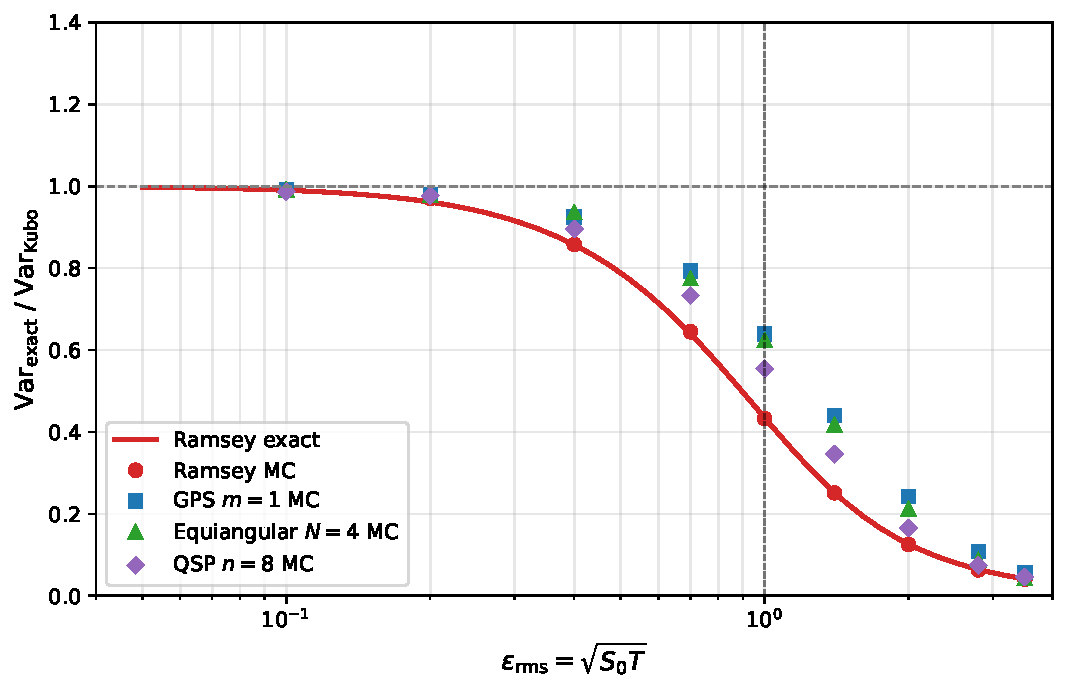
\includegraphics[width=0.48\textwidth]{figures/qubit_performance_plots/kubo_filter_comparison}
  \caption{Ratio of exact (analytic or Monte Carlo) variance to the linear-response
    Kubo prediction as a function of $\epsilon_{\rm rms} = \sqrt{S_0 T}$, for white
    noise $S_\beta(\omega)=S_0$ and $T=2\pi$.
    \emph{Red curve/circles}: Ramsey, exact analytic formula~\eqref{eq:ramsey_exact_var}
    and MC.
    \emph{Blue squares}: GPS $m=1$, Monte Carlo.
    Each Kubo baseline uses the analytic linear slope: $S_0 T/4$ (Ramsey) and
    $3\pi S_0/4$ (GPS $m=1$, Eq.~\eqref{eq:gps1_kubo}).
    The ratio is unity in the linear regime and falls below unity when the exact
    variance saturates while the Kubo prediction continues to grow linearly.
    The dashed vertical line marks $\epsilon_{\rm rms} = 1$.}
  \label{fig:kubo_validity}
\end{figure}


% ============================================================
\section{Protocol Performance Comparisons for Different Noise Spectra}
\label{sec:new_protocols}
% ============================================================

Here we examine additional noise scenarios of practical relevance: the mixed (two-corner)
noise model $S(\omega) = (1 + \omega_{c1}/|\omega|)\Theta(\omega_{c2}-|\omega|)$, which
interpolates between $1/f$ below $\omega_{c1}$, white between $\omega_{c1}$ and $\omega_{c2}$,
and zero above $\omega_{c2}$.  This models an LO with a $1/f$ corner at $\omega_{c1}$ and
a bandwidth cutoff at $\omega_{c2}$.

\placeholder{Add figure from plot\_mixed\_noise.py: FOM vs $\omega_{c2}$ for GPS $m=1,2,4,8,16$
and equiangular $N=4$ at several $\omega_{c1}$ values.
Key finding: GPS $m=8$ is optimal when $\omega_{c2} > 8$ and $\omega_{c1}=0$;
equiangular N=4 beats any single GPS by 5--10\%.}

% ============================================================
\section{Pulse Shaping for Improved Noise Suppression}
\label{sec:pulseshaping}
% ============================================================

In the linear response regime, the filter function is completely determined by the
path function $\Phi(\omega)$~\eqref{eq:Phi}.
This allows us to use pulse shaping---smooth modulation of $\Omega_j(t)$ and $\phi_j$---to
engineer $F_j^*(t)G_j(t)$ with a prescribed shape, achieving steeper roll-offs than
piecewise-constant sequences.

\subsection{Filter design via path-function engineering}

The key insight from Eq.~\eqref{eq:Fe} is that $\mathcal{F}_e(\omega) \propto |\Phi(\omega)|^2$
where $\Phi(\omega)$ is essentially the Fourier transform of the path function $F^*(t)G(t)$
along the Bloch sphere trajectory.
By the Paley--Wiener theorem \cite{}, the Fourier transform of a compactly supported
function in $[0,T]$ with $k$ continuous derivatives decays as $\omega^{-(k+1)}$ at
large $\omega$.
To achieve roll-off $\mathcal{F}_e \sim \omega^{-2(k+1)}$, we therefore require $k$
continuous derivatives of $F^*(t)G(t)$ at the pulse boundaries.

For standard equiangular pulses, $F^*(t)G(t)$ has jump discontinuities in its first
derivative at each pulse boundary ($k = 0$), giving $\mathcal{F}_e \sim \omega^{-2}$
(instantaneous limit) or $\omega^{-4}$ (finite-duration limit).
By using smoothly varying Rabi envelopes $\Omega(t)$ that join smoothly at boundaries,
one can achieve $k = 1$ ($\omega^{-6}$ roll-off) or higher.

\subsection{Smooth Rabi envelope sequences}

\placeholder{Derive the resulting $\Phi(\omega)$ analytically for the raised-cosine
envelope and show the $\omega^{-6}$ asymptotic decay.}

\placeholder{Figure: Pulse-shaping comparison. Left: Rabi envelopes $\Omega(t)$
for square pulse (standard GPS) and raised-cosine envelope.
Right: resulting filter functions $|\Phi(\omega)|^2$ on log-log scale, showing
$\omega^{-4}$ (square) vs $\omega^{-6}$ (raised cosine) roll-offs.
Include a reference $1/f^2$ noise spectrum.}

\subsection{Optimization via gradient descent}

The closed-form expression for $\Phi(\omega)$ enables efficient gradient-based
optimization.
For a parameterized family of pulse envelopes with parameters $\boldsymbol{\lambda}$
(Rabi amplitudes, phases, durations), the cost function
\be
  \mathcal{C}(\boldsymbol{\lambda}) = \int_{\omega_*}^\infty \frac{d\omega}{2\pi}\,
    S_\beta(\omega)\,|\Phi(\omega;\boldsymbol{\lambda})|^2
  \label{eq:cost_fn}
\ee
can be minimized by gradient descent using the analytic gradient
$\partial\mathcal{C}/\partial\lambda_k$.


% ============================================================
\section{Strongly Noisy Regime: Direct Clock Simulations}
\label{sec:strong_noise}
% ============================================================

When $\epsilon_{\rm rms} \gtrsim 1$, linear response theory breaks down and one must
return to direct time-domain simulation to assess clock performance.
In this regime the concept of a single filter function is no longer meaningful;
instead, clock performance is characterized by the Allan variance computed from
many realizations of the noisy clock cycle.

\subsection{Clock cycle model}
\label{sec:clock_model}

We model the full clock operation as follows.
At each cycle $k$ of duration $T$, the local oscillator has accumulated a phase error
$\phi_k = \int_{(k-1)T}^{kT} \delta_{\rm LO}(t)\,dt$ where $\delta_{\rm LO}(t)$ is the
LO frequency noise.
The atom experiences a detuning $\delta_k = \bar\delta + \delta_{\rm noise}^{(k)}$
where $\bar\delta$ is the slowly varying frequency offset (what the clock is locking to)
and $\delta_{\rm noise}^{(k)}$ is the fast noise accumulated during cycle $k$.

The clock servo updates the LO frequency based on the measured atomic signal $m_k$:
\be
  \bar\delta_{k+1} = \bar\delta_k - g\,\frac{m_k}{\mathcal{S}}\,,
  \label{eq:servo}
\ee
where $g$ is the servo gain.
The Allan variance is computed from the time record of $\bar\delta_k$ in the
standard way \cite{}.

\placeholder{Figure: Allan deviation $\sigma_y(\tau)$ for (a) two-level Ramsey,
(b) GPS-$m=4$, (c) GPS-$m=8$, (d) optimized pulsed QSP $n=5$,
for a $1/f^2$ noise model with $\beta_{\rm rms}$ in the nonlinear regime.
Show improvement in both short-$\tau$ (noise floor) and long-$\tau$ (drift) behavior.
Overlay the linear-response prediction (dashed) to show where it fails.}

\placeholder{Figure: Lock-in bandwidth (capture range) vs noise amplitude for
Ramsey vs QSP sequences, demonstrating improved dynamic range of QSP protocols.}

\subsection{Discussion: when does the GPS advantage persist?}

In the strongly noisy regime, the GPS advantage in DC sensitivity can be partially offset
by fringe-hopping---the servo locking to a neighboring fringe of the narrower GPS error signal.
\placeholder{Add analysis of fringe-hopping probability as a function of $\beta_{\rm rms}/\mathcal{S}$
for GPS-$m$ and Ramsey. Identify the crossover noise level above which GPS becomes
disadvantageous.}


% ============================================================
\section{Conclusions}
\label{sec:conclusion}
% ============================================================

We have introduced the temporal QSP formalism as a unified framework for understanding
and optimizing atomic clock performance under realistic noise environments.
The framework makes quantitative the connection between the algebraic structure of
pulse sequences---encoded in the Cayley--Klein amplitudes $F(t),G(t)$---and the two key
clock performance metrics: the per-shot frequency sensitivity $\mathcal{S}^2$ and the
Kubo noise filter function $\mathcal{F}_e(\omega)$.

The central analytical result, Eq.~\eqref{eq:gps_sens_result}, proves that all GPS
integer-cycle protocols at $\delta=0$ share the same DC sensitivity as Ramsey
($|\mathcal{S}|^2 = T^2/4$), so protocol comparisons reduce entirely to filter-function
differences.
The filter function has two contributions---from the coherence path $F^*G$ and the
population path $|G|^2$---and contrary to prior expectation, GPS filter functions are
\emph{peaked} (not nulled) at the Rabi frequency.

The numerical comparison of Table~\ref{tab:fom} establishes a quantitative hierarchy:
no single protocol is universally optimal, but pulsed QSP sequences achieve $3$--$7\times$
FOM improvement over all continuous-drive protocols for white and $1/f$ noise by
rediscovering CPMG-like spin-echo structures.
GPS $m=1$, by contrast, is nearly optimal for high-pass noise environments where its
filter function is concentrated below the noise cutoff.

Looking forward, the temporal QSP framework opens several directions:
the extension to multi-axis noise (simultaneous dephasing and amplitude noise),
gradient-based optimization of smooth pulse envelopes for steeper filter roll-off,
and the application to other quantum sensing platforms such as NV centers in diamond
and trapped-ion quantum sensors.
\placeholder{Add 2--3 sentences on most exciting near-term directions based on
group priorities.}


% ============================================================
\begin{acknowledgments}
\placeholder{Acknowledgments.}
\end{acknowledgments}

% ============================================================
\appendix

\section{Kubo Linear Response: Full Derivation}
\label{app:kubo}

This appendix derives the filter function formula~\eqref{eq:Fe} from first principles,
treating both the two-level qubit baseline and the three-level $\Lambda$ clock.

\subsection*{A1. Two-level qubit baseline}

For a single-qubit sensor with states $\{|g\rangle, |e\rangle\}$ and QSP control
propagator $U_{\rm QSP}(t)$ as in~\eqref{eq:u_qsp_poly}, the symmetric noise
Hamiltonian $H_\epsilon = \beta(t)\sigma_z^{ge}/2$ becomes in the toggling frame:
\begin{align}
  \tilde{H}(t) = U_{\rm QSP}^\dagger H_\epsilon U_{\rm QSP}
  = \frac{\beta(t)}{2}\begin{pmatrix}
      |F|^2-|G|^2 & -2iF^*G^* \\
      2iFG        & |G|^2-|F|^2
    \end{pmatrix}\,.
\end{align}
For initial state $|\psi_0\rangle = (|g\rangle+|e\rangle)/\sqrt{2}$ and
observable $M = \sigma_y^{ge}$, the Kubo formula gives
\be
  \langle\delta M^2\rangle = \int \frac{d\omega}{2\pi}\, S_\beta(\omega)\,
  \mathcal{F}^{(2L)}(\omega)\,,\quad
  \mathcal{F}^{(2L)}(\omega) = |\Phi(\omega)|^2\,,
\ee
where $\Phi(\omega) = \int_0^T F^*(t)G(t)\,e^{-i\omega t}\,dt$.
This is the standard dynamical-decoupling filter function \cite{Cywinski2008,Biercuk2009}.

\subsection*{A2. Three-level $\Lambda$ clock: two noise channels}

For the three-level Lambda system we have two independent noise channels:
\begin{itemize}
  \item \emph{Probe noise}: $H_e = \beta_e(t)|e\rangle\langle e|$ with PSD $S_e(\omega)$.
  \item \emph{Clock noise}: $H_m = \beta_m(t)|m\rangle\langle m|$ with PSD $S_m(\omega)$.
\end{itemize}
The QSP drive acts only on the $\{g,e\}$ probe subspace, leaving $|m\rangle$ unperturbed.
In the three-level toggling frame, the probe and clock noise operators become
\begin{align}
  \tilde{A}_e(t) &= |G|^2|g\rangle\langle g| + |F|^2|e\rangle\langle e|
     - iF^*G|g\rangle\langle e| + iFG^*|e\rangle\langle g|\,, \\
  \tilde{A}_m &= |m\rangle\langle m|\,.
\end{align}

\subsection*{A3. First-order signal response}

With $|\Psi\rangle = (|g\rangle + |m\rangle)/\sqrt{2}$ and
$M = \sigma_y^{gm} = -i|g\rangle\langle m| + i|m\rangle\langle g|$,
the commutator with the toggled probe noise evaluates to
\be
  \langle\Psi|[M, \tilde{A}_e(t)]|\Psi\rangle = \mathrm{Im}\bigl[F^*(t)G(t)\bigr]\,.
\ee
The $\tilde{A}_m$ contribution vanishes at first order for the equal-superposition state.
The first-order signal shift is $\langle\delta M\rangle = \int_0^T \beta_e(t)\,\mathrm{Im}[\phi(t)]\,dt$
where $\phi(t) \equiv F^*(t)G(t)$; this vanishes at $\delta=0$ as required.

\subsection*{A4. Second-order variance: probe noise}

Applying the Wiener--Khinchin theorem to the two-time noise correlator
$\langle\beta_e(t)\beta_e(t')\rangle = \int\frac{d\omega}{2\pi}\,S_e(\omega)\,e^{-i\omega(t-t')}$:
\be
  \langle\delta M^2\rangle_e = \int\frac{d\omega}{2\pi}\,S_e(\omega)
    \int_0^T\!\!\int_0^T\!\! dt\,dt'\,K_e(t,t')\,e^{-i\omega(t-t')}\,,
\ee
with $K_e(t,t') = \tfrac{1}{2}\,\mathrm{Re}[\phi(t)\,\phi^*(t')]$.
The factor $\tfrac{1}{2}$ (relative to the two-level formula) arises because the
probe Hamiltonian $\beta_e|e\rangle\langle e|$ shifts only one level, contributing
half the differential phase compared to the symmetric form $\beta\sigma_z/2$.
After Wiener--Khinchin the double integral factors:
\be
  \langle\delta M^2\rangle_e = \int\frac{d\omega}{2\pi}\,S_e(\omega)\cdot\tfrac{1}{2}|\Phi(\omega)|^2\,.
\ee

\subsection*{A5. Second-order variance: clock noise}

Clock noise $\beta_m(t)|m\rangle\langle m|$ phases the $|m\rangle$ component of the state
while leaving the probe subspace evolution unchanged.
After the QSP sequence the $|g\rangle$ amplitude at measurement is $F(T)/\sqrt{2}$;
the $|m\rangle$ amplitude acquires a stochastic phase $e^{-i\int_0^T\!\beta_m\,dt}/\sqrt{2}$.
The resulting variance contribution is:
\be
  \langle\delta M^2\rangle_m = \int\frac{d\omega}{2\pi}\,S_m(\omega)\cdot|\mathcal{X}(\omega)|^2\,,
\ee
where $\mathcal{X}(\omega) = \int_0^T |G(t)|^2\,e^{-i\omega t}\,dt$.

\subsection*{A6. Combined three-level filter function}

Summing probe and clock noise contributions with $S_e = S_m \equiv S_\beta$:
\be
  \langle\delta M^2\rangle = \int\frac{d\omega}{2\pi}\,S_\beta(\omega)\,\mathcal{F}_e(\omega)\,,
\ee
\be
  \mathcal{F}_e(\omega) = \tfrac{1}{2}|\Phi(\omega)|^2 + |\mathcal{X}(\omega)|^2\,,
\ee
recovering Eqs.~\eqref{eq:Fe}--\eqref{eq:Chi}.
The $\tfrac{1}{2}$ prefactor distinguishes the three-level result from the two-level
case: it reflects the asymmetric probe Hamiltonian $\delta|e\rangle\langle e|$ rather
than the symmetric form $\delta\sigma_z/2$.
The $|\mathcal{X}|^2$ term has no two-level analog; it captures the sensitivity of
the $\{g,m\}$ measurement to clock-transition fluctuations mediated by the
time-varying probe excited-state population $|G(t)|^2$.

\section{Two-Level Reduction}
\label{app:two_level_reduction}

Setting $|m\rangle \equiv |e\rangle$, $\beta_m \equiv \beta_e$, and taking
$M = \sigma_z^{ge}$ (so $m_z=1$, $m_x=m_y=0$) gives the standard qubit filter function:
\be
  \mathcal{F}^{(2L)}(\omega) = |\Phi(\omega)|^2\,,
\ee
where $\Phi(\omega) = \int_0^T F^*(t)G(t)\,e^{-i\omega t}\,dt$.
For a Ramsey interval ($\pi/2$--$\tau$--$\pi/2$ in the instantaneous limit),
$F^*(t)G(t) = (i/2)\sin(\omega_0\tau)\Theta(\tau<t<T-\tau)$ reduces to the standard result
$\mathcal{F}^{(2L)}_{\rm Ramsey}(\omega) = 4\sin^2(\omega T/2)/\omega^2$.

\section{Filter Functions for Standard Sequences}
\label{app:filter_functions}

\subsection*{C1. Ramsey sequence}

For two instantaneous $\pi/2$ pulses:
\be
  \mathcal{F}_{\rm Ramsey}(\omega) = \frac{4\sin^2(\omega T/2)}{\omega^2}\,.
\ee

\subsection*{C2. CPMG sequence ($n$ pulses, spacing $\tau$)}

Instantaneous pulses:
\be
  \mathcal{F}_{\rm CPMG}(\omega) = \frac{4}{\omega^2}
    \tan^2\!\left(\frac{\omega\tau}{2}\right)\sin^2\!\left(\frac{\omega n\tau}{2}\right)\,.
\ee

\subsection*{C3. GPS $m$-cycle sequence}

For $m$ identical equiangular cycles of total duration $T = m\tau_R$:
\be
  \Phi_{\rm GPS}(\omega) = \frac{1-e^{im\omega\tau_R}}{1-e^{i\omega\tau_R}}\,\Phi_{\rm cyc}(\omega)\,,
\ee
showing that the GPS filter function is a product of the single-cycle function
$|\Phi_{\rm cyc}(\omega)|^2$ and a standard multi-pulse interference factor.

\subsection*{C4. Roll-off behavior and pulse smoothness}

The high-frequency decay of $\mathcal{F}_e(\omega)$ is controlled by the regularity
of the path functions $\phi(t) = F^*(t)G(t)$ and $\chi(t) = |G(t)|^2$ at pulse
boundaries.
By repeated integration by parts, $k$ continuous derivatives of $\phi(t)$ give
$|\hat\Phi(\omega)| \leq C/|\omega|^{k+1}$ and $\mathcal{F}_e \sim \omega^{-2(k+1)}$
at large $\omega$:
\begin{center}
\begin{tabular}{lll}
\hline
Pulse type & Regularity $k$ & $\mathcal{F}_e$ roll-off \\
\hline
Instantaneous ($\tau_p \to 0$) & $-1$ & $\omega^{-2}$ \\
Square (piecewise constant)    & $0$  & $\omega^{-4}$ \\
Raised-cosine envelope         & $1$  & $\omega^{-6}$ \\
Gaussian-like                  & $\infty$ & faster than any power law \\
\hline
\end{tabular}
\end{center}
For standard equiangular sequences, $\phi(t)$ has discontinuous first derivatives at
pulse boundaries ($k=0$), giving the $\omega^{-4}$ roll-off observed numerically.
Smooth Rabi envelopes satisfying $\Omega(0)=\Omega(\tau)=0$ achieve $k\geq 1$ and
steeper roll-offs; see Sec.~\ref{sec:pulseshaping} and the raised-cosine construction
of Sec.~\ref{sec:pulseshaping}.

\section{Temporal QSP Polynomial Recurrences}
\label{app:recurrences}

During the $j$-th segment ($t_{j-1} < t \leq t_j$, Rabi frequency $\Omega_j$,
phase $\phi_j$, duration $\tau_j$):
\begin{align}
  F_j(t) &= \cos\tfrac{\theta_j(t)}{2}\,f_{j-1} - e^{-i\phi_j}\sin\tfrac{\theta_j(t)}{2}\,g_{j-1}^*\,, \\
  G_j(t) &= \cos\tfrac{\theta_j(t)}{2}\,g_{j-1} + e^{-i\phi_j}\sin\tfrac{\theta_j(t)}{2}\,f_{j-1}^*\,,
\end{align}
with $\theta_j(t) = \Omega_j(t-t_{j-1})$, $f_0 = 1$, $g_0 = 0$.

\section{GPS Sensitivity and Signal Formula}
\label{app:gps_sensitivity}

\subsection*{E1. Three-level propagator}

The Lambda system has levels $|g\rangle$, $|e\rangle$, $|m\rangle$ with probe
drive $H_{\rm drive} = \tfrac{\Omega}{2}(|g\rangle\langle e|+|e\rangle\langle g|)$
and detuning Hamiltonian $H_\delta = \delta|e\rangle\langle e|$.
The form $H_\delta = \delta|e\rangle\langle e|$ is \emph{not} traceless in the
$\{g,e\}$ probe subspace; it generates a global probe phase $e^{-i\delta\tau/2}$
relative to $|m\rangle$ over each segment of duration $\tau$.
For a single continuous drive of duration $T$ at detuning $\delta$, the full
three-level propagator is
\be
  U(\delta, T) = e^{-i\delta T/2}
  \begin{pmatrix}
    f(\delta,T) & ig(\delta,T) & 0 \\
    ig^*(\delta,T) & f^*(\delta,T) & 0 \\
    0 & 0 & e^{i\delta T/2}
  \end{pmatrix},
  \label{eq:3level_prop_app}
\ee
where $f$, $g$ are the Cayley--Klein amplitudes for the SU(2) rotation in the probe
subspace under the traceless part of $H_\delta + H_{\rm drive}$:
\begin{align}
  f(\delta,T) &= \cos\!\left(\frac{\Omega_R T}{2}\right)
    + i\frac{\delta}{\Omega_R}\sin\!\left(\frac{\Omega_R T}{2}\right), \\
  g(\delta,T) &= -i\frac{\Omega}{\Omega_R}\sin\!\left(\frac{\Omega_R T}{2}\right),
\end{align}
with $\Omega_R = \sqrt{\Omega^2 + \delta^2}$.

\subsection*{E2. GPS clock signal}

The initial clock state is $|\psi_0\rangle = (|g\rangle+|m\rangle)/\sqrt{2}$ and
the measurement operator is $M = \sigma_y^{gm} = -i|g\rangle\langle m|+i|m\rangle\langle g|$.
After the GPS drive, $|g\rangle$ evolves to $U|g\rangle$ while $|m\rangle$ is
unaffected (the lower-right block of~\eqref{eq:3level_prop_app} contributes only a phase).
The clock signal is:
\begin{align}
  S(\delta)
  &= \langle\psi_0|U^\dagger M\,U|\psi_0\rangle
   = \mathrm{Im}\!\left[e^{i\delta T/2}f^*(\delta,T)\right].
\end{align}
Substituting the explicit form of $f$ gives Eq.~\eqref{eq:gps_signal} of the main text:
\be
  S(\delta) = \sin\!\left(\frac{\delta T}{2}\right)\cos\!\left(\frac{\Omega_R T}{2}\right)
            - \frac{\delta}{\Omega_R}\cos\!\left(\frac{\delta T}{2}\right)
              \sin\!\left(\frac{\Omega_R T}{2}\right).
  \label{eq:gps_signal_app}
\ee
The alternative probe-subspace-traceless formula $S = (\delta/\Omega_R)\sin(\Omega_R T/2)$
omits the global probe phase and gives incorrect signal predictions away from $\delta = 0$.

\subsection*{E3. DC sensitivity: all GPS-$m$ match Ramsey}

Differentiating Eq.~\eqref{eq:gps_signal_app} with respect to $\delta$ and
evaluating at $\delta=0$ (where $\Omega_R\to\Omega$, $\partial_\delta\Omega_R\to 0$):
\begin{align}
  \partial_\delta S\big|_{\delta=0}
  &= \frac{T}{2}\cos\!\left(\frac{\Omega T}{2}\right)
   - \frac{\sin(\Omega T/2)}{\Omega}\,.
\end{align}
For GPS-$m$ with $\Omega T = 2\pi m$: $\sin(m\pi) = 0$ and $\cos(m\pi) = (-1)^m$, so
\be
  \partial_\delta S\big|_{\delta=0}^{\rm GPS\text{-}m} = \frac{(-1)^m T}{2}\,,
  \qquad
  \left|\partial_\delta S\big|_{\delta=0}\right|^2 = \frac{T^2}{4}\quad\forall\,m\,.
\ee
This is Eq.~\eqref{eq:gps_sens_result}.
The squared DC sensitivity $T^2/4 = \pi^2$ (for $T=2\pi$) is the same for all $m$ and
equals the Ramsey sensitivity; all FOM differences between GPS protocols arise from
$\mathcal{F}_e(\omega)$, not $\mathcal{S}^2$.
Finite-difference verification ($\Delta\delta=10^{-5}$) agrees with this analytic
result to $<0.1\%$ for $m = 1, 2, 4, 8$.

\subsection*{E4. GPS filter function structure}

At $\delta=0$, the GPS-$m$ CK amplitudes evolve as $F(t) = \cos(\Omega t/2)$,
$G(t) = -i\sin(\Omega t/2)$, giving path functions
\be
  \phi(t) = F^*(t)G(t) = \tfrac{i}{2}\sin(\Omega t)\,,\qquad
  |G(t)|^2 = \tfrac{1}{2}[1-\cos(\Omega t)]\,.
\ee
The Fourier transforms are peaked near $\omega = \Omega$ and $2\Omega$, so
$\mathcal{F}_e(\omega) = \tfrac{1}{2}|\Phi|^2 + |\mathcal{X}|^2$ is
\emph{peaked} at the drive frequency---not nulled there.
This corrects the prediction from the probe-subspace-traceless Hamiltonian,
which spuriously generates nulls at Rabi harmonics.
Protocols with $\Omega < \omega_c$ are effectively transparent to band-limited
high-pass noise, explaining the large FOM of GPS-$m=1$ under high-pass noise.

\section{Pulse Sequence Optimization}
\label{app:optimization}

\subsection*{F1. Optimization objective}

All protocols are optimized with respect to the FOM~\eqref{eq:fom}.
Since the DC sensitivity $|\partial_\delta\langle M\rangle|_{\delta=0}^2$ is fixed
at $T^2/4$ for all protocols at $\delta=0$ (Eq.~\eqref{eq:gps_sens_result}),
maximizing FOM is equivalent to minimizing the Kubo denominator
$\mathcal{C}(\boldsymbol{\lambda}) = \int_0^\infty \mathcal{F}_e(\omega;\boldsymbol{\lambda})\,S(\omega)\,d\omega/(2\pi)$,
evaluated via FFT (Sec.~\ref{sec:numerics}).

\subsection*{F2. Equiangular $N$-segment optimization}

The free parameters are $(\Omega, \phi_2,\ldots,\phi_N)$, with
$\Omega\in(0, \Omega_{\rm max}]$ and $\phi_k\in[0,2\pi)$.
The optimization proceeds in two stages:
\begin{enumerate}
  \item \emph{Global search}: Differential Evolution (DE) with population size 20,
        maximum 500 generations, ``best/1/bin'' mutation, crossover probability 0.7,
        over $\Omega\in[\pi/(10T), N\pi/T]$ and $\phi_k\in[0,2\pi)$.
        Twelve random-seed restarts guard against local minima.
  \item \emph{Local polishing}: L-BFGS-B from the best DE solution,
        gradient by central finite differences ($\epsilon=10^{-5}$),
        convergence at $\Delta\mathcal{C}<10^{-9}$, $|\nabla\mathcal{C}|<10^{-7}$.
\end{enumerate}
For white noise ($N=4$), the optimal parameters are
$\Omega^* T \approx 7.6$\,rad, $\boldsymbol{\phi}^*\approx[0,1.44,0.38,1.11]$\,rad.

\subsection*{F3. Pulsed QSP optimization}

The free parameters are $(\theta_1,\ldots,\theta_n, \phi_2,\ldots,\phi_n)$
($2n-1$ total; $\phi_1=0$ by gauge), with $\theta_j\in[0.01\pi,\pi]$ and
$\phi_j\in[0,2\pi)$.
The upper bound $\theta_j\leq\pi$ restricts each pulse to at most a half Rabi cycle.
The free-evolution gap is determined by $\tau_{\rm free} = (T-\sum_j\theta_j/\Omega_{\rm fast})/(n-1)$;
feasibility ($\tau_{\rm free}>0$) is always satisfied for $\Omega_{\rm fast}T = 40\pi^2$.

The same two-stage DE\,+\,L-BFGS-B procedure is used, with budgets scaled by $2n-1$:
\begin{center}
\begin{tabular}{cccc}
\toprule
$n$ & Free params & DE pop & DE maxiter \\
\midrule
3  & 5  & 10 & 150 \\
5  & 9  & 10 & 120 \\
9  & 17 & 8  & 80  \\
\bottomrule
\end{tabular}
\end{center}
Multiple restarts (4 for $n=3$, 3 for $n=5$, 2 for $n=9$) are performed and
the best result is refined by L-BFGS-B.

All filter functions in the objective use $N_{\rm FFT}=1024$, zero-padding $\times 2$;
final FOMs in Table~\ref{tab:fom} are recomputed at $N_{\rm FFT}=4096$, zero-padding $\times 4$.

\bibliography{ref}
\end{document}
